\subsection{Channel models, surface size and long delay spread}\label{sec:res-chan}
\emph{3GPP channels.} Table~\ref{tab:tdl} uses the TR~38.901 TDL models. At 30\,ns, as in the
anchor paper, two pilot symbols suffice (gap $\le0.14$ at 20\,dB). With realistic delay spreads
the default setting, designed for the six-path model, breaks: TDL channels have 14--24 taps from
different directions. Matching the delay window to the delay spread
($\tau_{\max}=\min(T_{\rm cp},10\times$DS$)$) and raising the rank to 16 fixes 100\,ns with eight
pilot symbols: gap 0.08--0.24\,bit/s/Hz at 20\,dB. The rank barely matters (8, 16 and 32 give
the same within 0.1); the number of pilots is the lever, because a longer delay window means more
unknowns (Table~\ref{tab:unknowns}). We note a correction this exposed: an earlier robustness check
to 100\,ns, made with the six-path model, was optimistic for standard channels.

\begin{table}[!htbp]\centering
\caption{Gap (bit/s/Hz) on 3GPP TDL channels at 20\,dB (30\,dB in brackets), window matched to the delay spread, ranges over ranks 8/16/32, 6 channels.}\label{tab:tdl}
\begin{tabular}{lccc}\toprule
 & $N_p=2$ & $N_p=4$ & $N_p=8$ \\\midrule
TDL-A, 100\,ns & 0.69--0.76 (2.5--2.8) & 0.21--0.32 (0.8--0.9) & \textbf{0.08--0.09} (0.24--0.27) \\
TDL-C, 100\,ns & 0.47--0.50 (1.7--1.9) & 0.17--0.24 (0.6--0.8) & \textbf{0.09--0.10} (0.18--0.26) \\
TDL-D, 100\,ns & 0.65--0.69 (2.1--2.3) & 0.31--0.37 (1.3--1.4) & \textbf{0.23--0.24} (0.85--0.95) \\
TDL-A/C/D, 300\,ns & 1.1--1.5 (3.4--4.7) & 0.6--1.1 (2.6--3.3) & 0.35--0.92 (1.4--2.3) \\\bottomrule
\end{tabular}
\end{table}

\emph{Surface size and near field.} With TDL-C at 30\,ns, $Q=64$, 256 and 1024 elements give a gap
of 0.06--0.11 / 0.17--0.25\,bit/s/Hz at 20/30\,dB with two pilot symbols: the unknowns do not grow
with $Q$ (Corollary~\ref{cor:lowrank}). With $Q=1024$ (1.3\,m aperture, Fraunhofer distance about 40\,m)
and the TDL-D line-of-sight path computed from exact element distances, a user at 3, 10 and 30\,m
sees a gap of 0.09--0.18 / 0.38--0.60 (Fig.~\ref{fig:tdl}).

\textbf{Validity warning for 300\,ns.} The cyclic-prefix condition (A2) applies to the \emph{cascade}
of both hops, and our generator gives each hop the full TDL profile. The maximum cascaded delay is
$2\times9.66$, $2\times8.65$ and $2\times12.5$ times the delay spread for TDL-A, C and D: 5.8, 5.2 and
7.5\,$\mu$s at 300\,ns, all beyond the 2.34\,$\mu$s prefix (and 2.5\,$\mu$s for TDL-D at 100\,ns, a weak
violation through taps below $-27$\,dB). The ground truth~\eqref{eq:io} assumes the prefix condition and
omits the resulting inter-symbol interference, so \emph{all 300\,ns results below are physically invalid}
and are kept only as a record; they are not claims of this paper. A valid long-delay test needs
a realistic split (e.g. a short line-of-sight BS--RIS hop) and is future work.

\emph{300\,ns (invalid, see above): learning the static side.} At 300\,ns, eight pilot symbols are not enough. With
Algorithm~\ref{alg:learn} (input side learned from 100 frames of other users or earlier positions,
$r=Q=16$), TDL-A and TDL-C reach a gap of 0.23 and 0.26\,bit/s/Hz at 20\,dB, against 0.36 and 0.46 from
one frame, and the gap at 30\,dB halves (Table~\ref{tab:300}, Fig.~\ref{fig:300}). The pre-registered
criterion (all three models $\le0.3$ at 20\,dB) nevertheless \emph{failed}, on TDL-D: it fails even when
the true static side is given (0.56), because at 300\,ns TDL-D has taps up to $12.5\times300$\,ns
$=3.8\,\mu$s, beyond the 2.34\,$\mu$s cyclic prefix (A2). Taps beyond the prefix carry about $-20$\,dB of
power, which no prefix-limited delay window can represent; a real system would switch to an extended
prefix. Two earlier versions of the learning step also failed their criteria: initializing from a single
frame gave no gain over one frame (0.37 vs 0.33 on TDL-A), and 30 frames gave 0.31. The stacked
initialization, the learned prior and 100 frames were each needed. One hundred frames is a short time
compared with the coherence of the BS--RIS hop, which is static for minutes.

\begin{table}[!htbp]\centering
\caption{300\,ns delay spread, eight pilot symbols: gap (bit/s/Hz) at 20 / 30\,dB, 6 channels.}\label{tab:300}
\begin{tabular}{lccc}\toprule
 & one frame & learned side, 100 frames & true static side \\\midrule
TDL-A & 0.36 / 1.91 & \textbf{0.23} / 0.85 & 0.12 / 0.37 \\
TDL-C & 0.46 / 1.84 & \textbf{0.26} / 0.99 & 0.12 / 0.32 \\
TDL-D & 0.85 / 2.74 & 0.64 / 2.89 & 0.56 / 1.61 \\\bottomrule
\end{tabular}
\end{table}
\begin{figure}[!htbp]\centering
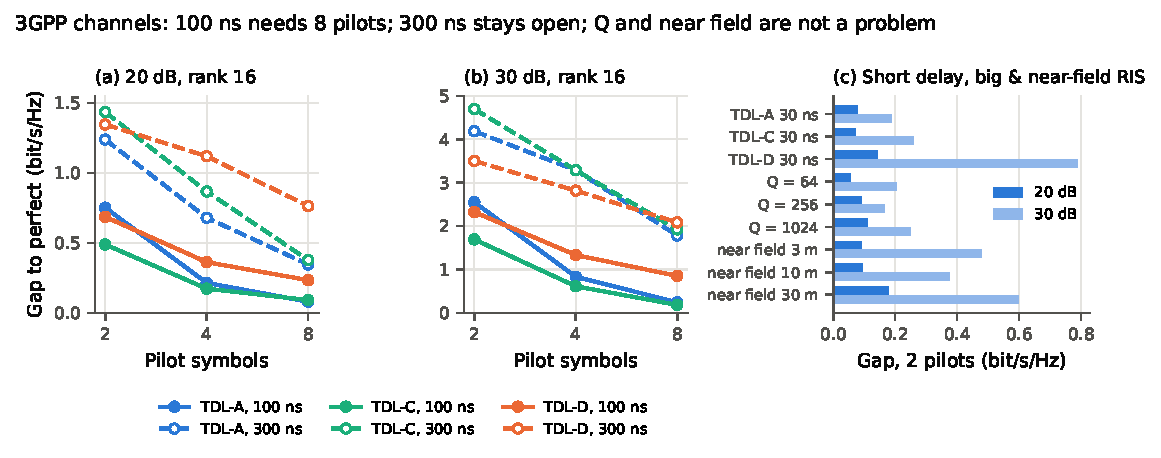
\includegraphics[width=\columnwidth]{fig14_tdl_channels.pdf}
\caption{3GPP channels: gap versus pilot symbols at 100 and 300\,ns; short delay spread, large and near-field surfaces.}
\label{fig:tdl}\end{figure}
\begin{figure}[!htbp]\centering
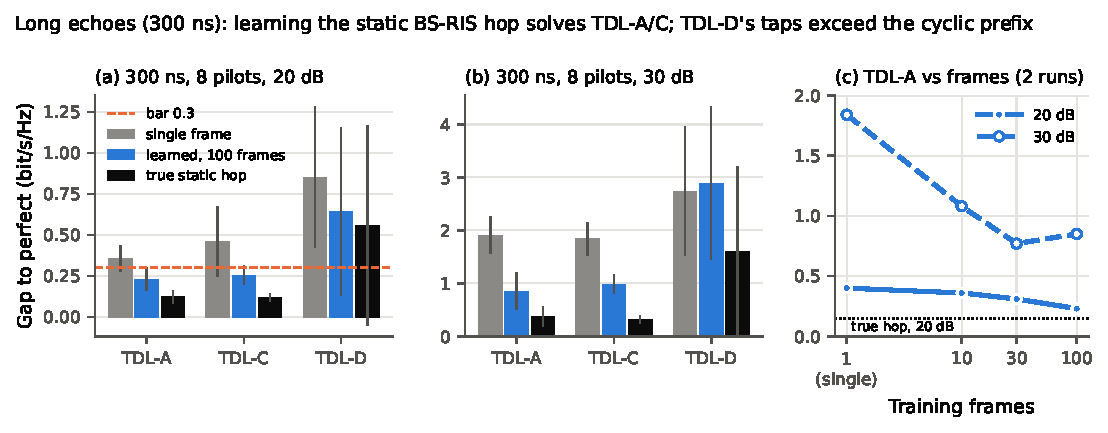
\includegraphics[width=\columnwidth]{fig21_two_timescale.pdf}
\caption{Learning the static BS--RIS side at 300\,ns delay spread.}
\label{fig:300}\end{figure}

\subsection{Timing knowledge and blind offset recovery}\label{sec:res-timing}
\emph{Sensitivity.} With the nominal timing, an unknown common offset of 0.02 slot (83\,ns) costs
4.3/11.3\,dB at 20/30\,dB, and 0.2 slot costs 15.1/25.3\,dB (Fig.~\ref{fig:timing}). The receiver must
therefore either know or estimate the offset.

\emph{Residual-based recovery.} Scanning the offset and keeping the smallest pilot residual recovers
on-grid offsets exactly (0.05, 0.20, 0.40 slot; loss within 0.03\,dB of known timing). For off-grid
offsets (uniform in $\pm0.5$ slot, grid plus golden section, 12 channels) it works at 20\,dB (0.20\,dB
vs 0.19 known) but fails at 30\,dB: rms error 0.021 slot (87\,ns), loss 4.80\,dB against 0.41\,dB
known. Refining with the full estimator and with decided data did not help (3.78\,dB). The error
grew from 20 to 30\,dB, which indicates an ambiguity rather than noise, as Proposition~\ref{prop:offset}
predicts.

\emph{A failed idea.} Since an offset is a delay, a delay window widened by a guard should absorb it
with no search. It does not (criterion failed): at 30\,dB, for offsets up to 83\,ns, the guard
window loses 2.32\,dB against 1.76\,dB without it (0.39 known); for offsets up to 208\,ns it improves
12.3 to 9.2\,dB, far from 0.28. A diagnostic showed why: the shifted responses were representable
in the plain basis already (projection error $10^{-4}$); the issue is the prior, which shrinks the
improbable shifted responses, and a wider window spreads the prior over more dimensions.

\emph{Evidence-based recovery} (Algorithm~\ref{alg:offset}) uses exactly that prior. On the same
channels and offsets as the residual search, it gives an rms error of 0.0012 slot (5\,ns) at both
20 and 30\,dB (measured against the generator's offset, which shares the delay reference of the
prior; by Proposition~\ref{prop:offset} only the rate loss is reference-free), and losses of 0.25 and 0.40\,dB against 0.25 and 0.41\,dB with the offset known
(Table~\ref{tab:timing}, Fig.~\ref{fig:blind}); the pre-registered criterion (within 1\,dB of known at
30\,dB) passed. Every one of the 12 channels at 30\,dB lies on the known-timing line, including the
three where the residual search lost more than 10\,dB.

\begin{table}[!htbp]\centering
\caption{Blind recovery of an off-grid clock offset (12 channels, $N_p=2$).}\label{tab:timing}
\begin{tabular}{lcccc}\toprule
 & \multicolumn{2}{c}{rms error (slot)} & \multicolumn{2}{c}{loss (dB)} \\
 & 20\,dB & 30\,dB & 20\,dB & 30\,dB \\\midrule
Residual search & 0.0045 & 0.0210 & 0.57 & 4.80 \\
\textbf{Evidence search (Alg.~\ref{alg:offset})} & \textbf{0.0011} & \textbf{0.0012} & \textbf{0.25} & \textbf{0.40} \\
Offset known & -- & -- & 0.25 & 0.41 \\\bottomrule
\end{tabular}
\end{table}

\emph{Jitter.} Random jitter of individual switching edges changes the pattern's shape, not only
its delay, so it is not absorbed. It must stay below about 20\,ns rms for 20\,dB operation and 4\,ns for
30\,dB (loss at 4/8/21\,ns: 0.24/0.40/0.97\,dB at 20\,dB, 0.94/2.05/5.91\,dB at 30\,dB). Microcontroller
and FPGA clocks have jitter in the picosecond range.

\begin{figure}[!htbp]\centering
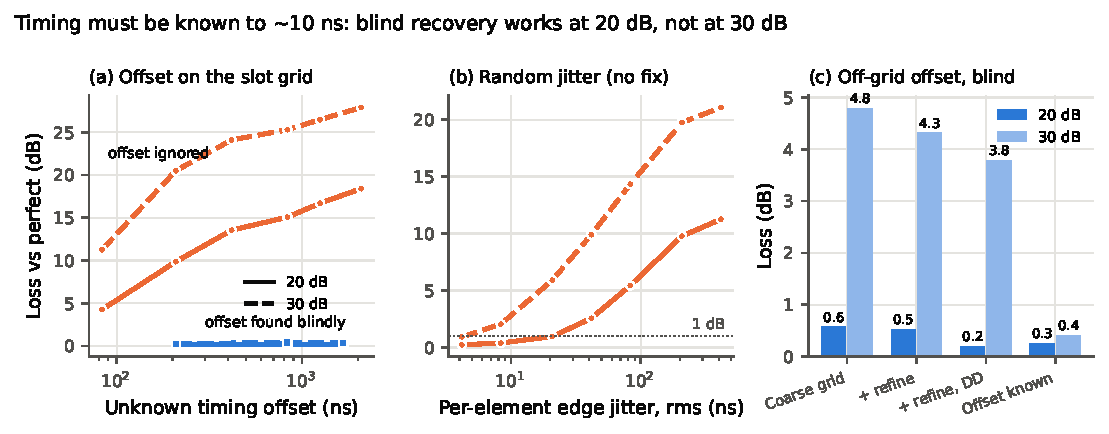
\includegraphics[width=\columnwidth]{fig12_timing.pdf}
\caption{Timing: offset sensitivity, jitter, residual-based off-grid recovery.}
\label{fig:timing}\end{figure}
\begin{figure}[!htbp]\centering
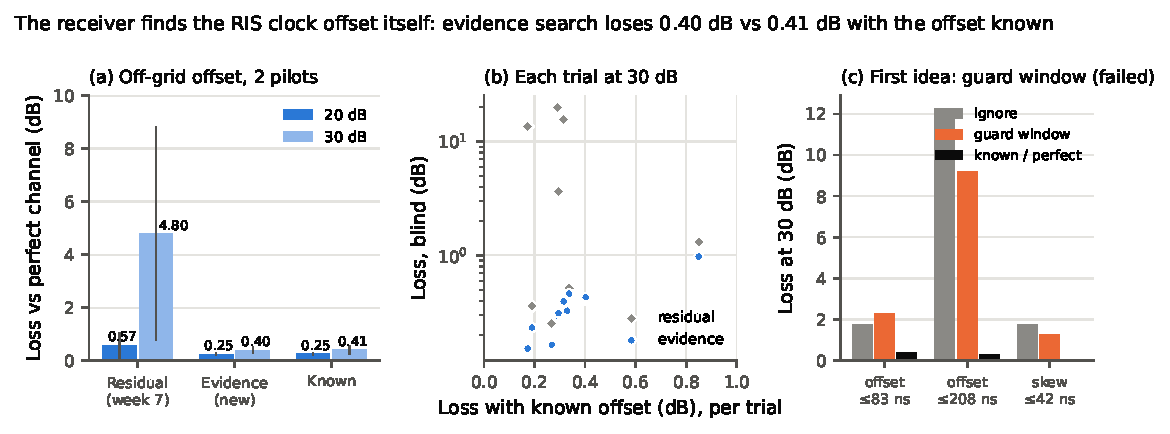
\includegraphics[width=\columnwidth]{fig20_blind_timing.pdf}
\caption{Evidence-based blind offset recovery; per-channel losses; the failed guard-window idea.}
\label{fig:blind}\end{figure}

\subsection{Hardware impairments}\label{sec:res-hw}
\emph{Element spread.} Random resonance spread of 5--20\,MHz between elements, with $\pm5\%$ loss
spread, costs 0.20--0.28 / 0.28--0.46\,dB at 20/30\,dB: the timing-only estimator never assumed
identical elements.

\emph{Switching transients.} A linear ramp between states with rise time $\rho$ (fraction of a
slot) costs up to 3.9/11.7\,dB if ignored. Building the kernels from a ramped waveform with $\rho$
calibrated once, or chosen blindly by the smallest pilot residual on a grid, brings this to
0.21--0.43 / 0.36--0.61\,dB for $\rho=0.05$--0.3; the blind estimate is within 0.03 of the true rise time.

\emph{Carrier frequency offset.} A residual CFO of 0.5/1/2/5\% of the spacing costs
0.26/0.32/0.52/1.70\,dB at 20\,dB and 0.72/1.00/2.45/7.50\,dB at 30\,dB: residual CFO must stay
below about 1\%, as standard OFDM synchronization provides.

\emph{Phase noise.} With a continuous Wiener phase over pilots and data and common-phase removal per
symbol, the fair reference is a genie that knows the channel but not the phase noise. Our receiver
adds 0.37, 0.52, 0.90 and 1.20\,dB to that reference at 20\,dB for 10, 100, 1000 and 10\,000\,Hz
linewidth (0.42, 0.99, 1.37, 1.38\,dB at 30\,dB). The pre-registered criterion (within 0.5\,dB at
$\le1$\,kHz, 20\,dB) failed at 1\,kHz and was borderline at 100\,Hz: the pilots are corrupted too.
Most of the loss, however, is the generic phase-noise ICI that any receiver suffers (the genie
itself falls from 6.63 to 4.72\,bit/s/Hz at 1\,kHz). Requirement: linewidth below about 100\,Hz at
30\,kHz spacing, or standard phase tracking (Fig.~\ref{fig:hw}).

\begin{figure}[!htbp]\centering
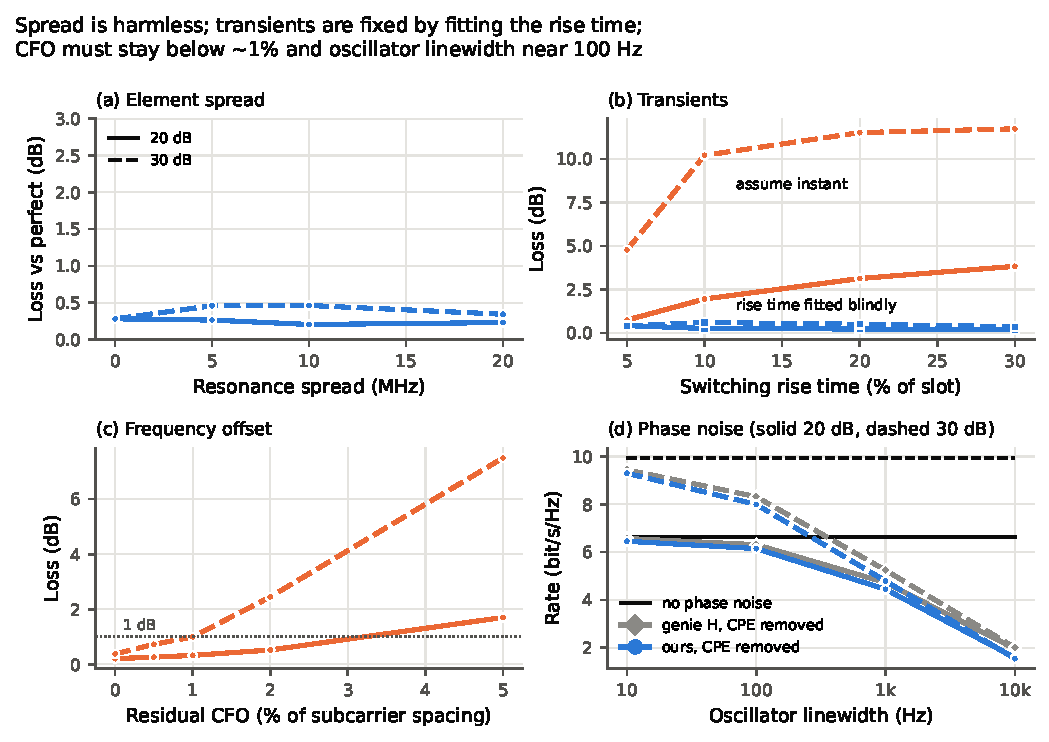
\includegraphics[width=0.85\columnwidth]{fig13_hardware.pdf}
\caption{Element spread, switching transients, CFO and phase noise.}
\label{fig:hw}\end{figure}

\subsection{Direct path, multiple panels and interference}\label{sec:res-direct}
\emph{Unblocked direct path.} A direct path at $-20$ to $+10$\,dB relative to the RIS path needs no
change to the estimator, by Corollary~\ref{cor:groups}(iii): at 0\,dB, 5.28/8.13 against 5.39/8.49
with perfect knowledge (an explicit direct-path term gives the same numbers). The one-tap receiver
improves with a strong direct path (2.9--3.1\,bit/s/Hz at $+10$\,dB) but stays far below.

\emph{Two panels.} Two TM-RIS panels with independent channels and different patterns ($G=2$): 5.54/8.67
against 5.64/8.86. A receiver that models only one panel collapses to 1.15: the receiver must know the
timing of every panel (A1).

\emph{Interference.} An unknown OFDM interferer through its own channel, treated as noise, at
SIR 20/10/0\,dB: within 0.03--0.17\,bit/s/Hz of perfect knowledge at every SIR; interference limits
both equally (Fig.~\ref{fig:direct}).

\begin{figure}[!htbp]\centering
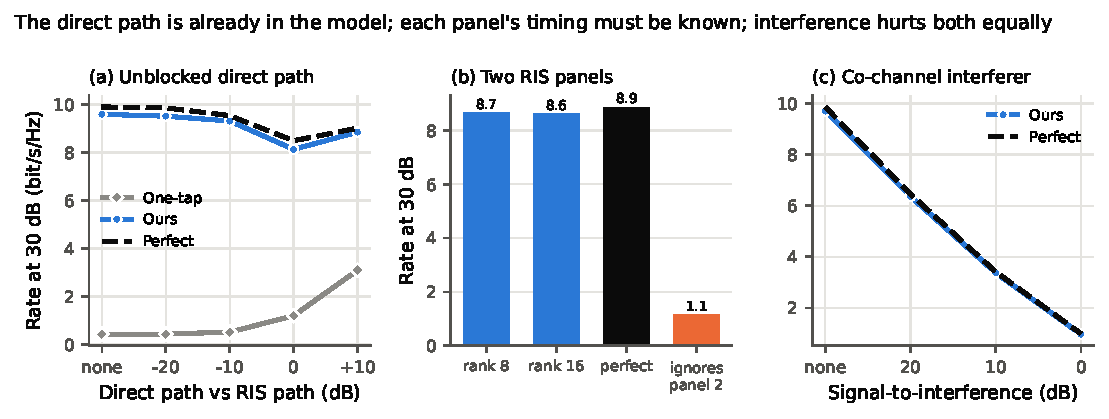
\includegraphics[width=\columnwidth]{fig17_direct_link.pdf}
\caption{Unblocked direct path, two panels, co-channel interference.}
\label{fig:direct}\end{figure}

\subsection{Pilot design}\label{sec:res-pilot}
With the same number of pilot resource elements (512) and energy: two full pilot symbols give
6.49/9.71; comb pilots on every second subcarrier over four symbols with the other resource elements
\emph{empty}, as NR DMRS allows, give 6.52/9.79; every fourth subcarrier over eight symbols, 6.51/9.77.
With \emph{data} in the gaps, the switching leaks data into the pilot bins and the rate falls to
4.79/5.10; one DD pass recovers 6.36/8.82. Design rule: comb pilots work if their neighbours are empty.

\subsection{Mobility, coherence time and pilot overhead}\label{sec:res-mob}
\emph{Coherence.} Only the RIS--user hop moves. The coherence time $T_c=0.423/f_D$ with
$f_D=vf_c/c$ is 42.4\,ms (1188 symbols) at 3\,km/h, 4.24\,ms (119 symbols) at 30\,km/h and 1.06\,ms
(30 symbols) at 120\,km/h. Doppler mixing within a symbol is $-60$, $-47$ and $-34$\,dB relative to the
signal at these speeds (0, 0.008 and 0.19\,bit/s/Hz at 30\,dB), so the main effect is the ageing of
the estimate. With one estimate reused (per-subcarrier gain metric), the gap at 20\,dB stays below 0.1\,bit/s/Hz
for more than 300 symbols at 3\,km/h, reaches 0.26 after 40 symbols at 30\,km/h (20\,dB), and 0.32 after 10
symbols at 120\,km/h (Fig.~\ref{fig:mob}).

\emph{Two failed tracking receivers.} Tracking $\bm U$ symbol by symbol from decisions, with the input
side learned, made things worse than reusing the pilot estimate (average gap over 40 symbols at 20\,dB:
0.52 against 0.28); a proper Kalman filter with propagated covariance also failed (0.46). Wrong decisions
accumulate after about ten symbols, and at 30\,dB even the first symbol after the pilots has a gap of
0.44--0.52 for every receiver, because the in-symbol Doppler mixing at 120\,km/h is not in our model.
Fast users therefore need frequent pilots, which the overhead analysis quantifies.

\emph{Net throughput.} Table~\ref{tab:overhead} and Fig.~\ref{fig:overhead} give the net rate after pilot
overhead with the refresh interval and pilot count optimized per case. After paying for its pilots,
the proposed receiver beats the best CE-BEM in every one of the 24 cases, by 1.1--4.8\,bit/s/Hz (median 2.7). On the 3GPP
channels at 20\,dB it needs 5--7\% overhead at 3\,km/h, 5--10\% at 30\,km/h and 12\% at 120\,km/h (one pilot
symbol every eight). Slow channels with long echoes prefer several pilot symbols per refresh (four, on
TDL at walking speed); fast channels prefer one pilot symbol refreshed often. The six-path model needs
less overhead at speed (1--3\% at 20\,dB) because its dominant line-of-sight path makes the Doppler mostly a common
phase, which tracking removes; the non-line-of-sight TDL numbers are the realistic ones. Without any phase
tracking, 120\,km/h requires about 25\% overhead.

\begin{table}[!htbp]\centering
\caption{Net throughput (bit/s/Hz) after pilot overhead, refresh interval and pilot count optimized per case; in brackets: pilot symbols / block length. Ours with common-phase tracking (main), its range from no tracking to a per-subcarrier genie, the best CE-BEM (best harmonic range and pilot count, same tracking), one-tap, and perfect knowledge without pilots. Shared-path: 8 channels; TDL: 4 channels per point. CE-BEM on TDL is limited to $|h|\le40$.}\label{tab:overhead}
\begin{tabular}{llcccccc}\toprule
Channel & km/h & SNR & ours & ours range & CE-BEM & one-tap & perfect\\\midrule
Shared-path, 30\,ns & 3 & 20 & 6.28 (2/120) & 5.98--6.33 & 5.14 (32/320) & 0.38 & 6.49\\
Shared-path, 30\,ns & 3 & 30 & 9.29 (2/80) & 8.43--9.47 & 6.87 (16/240) & 0.42 & 9.79\\
Shared-path, 30\,ns & 30 & 20 & 6.13 (1/40) & 5.38--6.53 & 4.83 (16/240) & 0.39 & 6.60\\
Shared-path, 30\,ns & 30 & 30 & 8.93 (1/30) & 7.21--9.40 & 6.02 (16/240) & 0.42 & 9.90\\
Shared-path, 30\,ns & 120 & 20 & 5.59 (1/160) & 3.70--6.23 & 3.43 (8/320) & 0.40 & 6.49\\
Shared-path, 30\,ns & 120 & 30 & 7.55 (1/10) & 4.40--8.56 & 2.96 (16/320) & 0.43 & 9.78\\
\midrule
TDL-A, 100\,ns & 3 & 20 & 5.05 (4/60) & 4.91--5.34 & 3.44 (16/160) & 0.33 & 5.91\\
TDL-A, 100\,ns & 3 & 30 & 6.61 (4/40) & 6.50--7.03 & 3.25 (16/120) & 0.39 & 8.94\\
TDL-A, 100\,ns & 30 & 20 & 4.70 (1/10) & 4.47--5.29 & 2.25 (8/40) & 0.34 & 6.31\\
TDL-A, 100\,ns & 30 & 30 & 5.89 (2/15) & 5.41--6.96 & 1.93 (16/60) & 0.40 & 9.54\\
TDL-A, 100\,ns & 120 & 20 & 4.26 (1/8) & 3.65--4.97 & 1.53 (16/240) & 0.34 & 6.28\\
TDL-A, 100\,ns & 120 & 30 & 5.09 (1/6) & 4.34--6.08 & 1.24 (16/240) & 0.38 & 9.51\\
\midrule
TDL-C, 100\,ns & 3 & 20 & 5.71 (4/80) & 5.55--6.02 & 3.70 (16/240) & 0.38 & 6.34\\
TDL-C, 100\,ns & 3 & 30 & 8.05 (4/60) & 7.61--8.60 & 3.33 (16/240) & 0.42 & 9.58\\
TDL-C, 100\,ns & 30 & 20 & 4.81 (1/10) & 4.69--5.20 & 2.10 (8/40) & 0.33 & 5.95\\
TDL-C, 100\,ns & 30 & 30 & 6.03 (1/8) & 5.80--6.73 & 1.73 (8/30) & 0.37 & 9.13\\
TDL-C, 100\,ns & 120 & 20 & 4.34 (1/8) & 3.65--4.95 & 1.66 (16/320) & 0.33 & 6.07\\
TDL-C, 100\,ns & 120 & 30 & 5.37 (1/6) & 4.39--6.39 & 1.39 (16/320) & 0.40 & 9.30\\
\midrule
TDL-D, 100\,ns & 3 & 20 & 5.58 (4/80) & 5.22--5.77 & 3.63 (16/160) & 0.39 & 6.25\\
TDL-D, 100\,ns & 3 & 30 & 8.06 (2/60) & 7.46--8.51 & 3.26 (16/160) & 0.40 & 9.51\\
TDL-D, 100\,ns & 30 & 20 & 5.06 (1/20) & 4.53--5.60 & 2.88 (32/320) & 0.37 & 6.49\\
TDL-D, 100\,ns & 30 & 30 & 7.06 (1/15) & 5.96--7.73 & 2.55 (16/320) & 0.42 & 9.75\\
TDL-D, 100\,ns & 120 & 20 & 3.91 (1/8) & 3.10--4.74 & 1.64 (16/160) & 0.32 & 6.13\\
TDL-D, 100\,ns & 120 & 30 & 4.94 (1/8) & 3.66--5.51 & 1.36 (16/160) & 0.34 & 9.32\\
\bottomrule
\end{tabular}
\end{table}

\begin{figure}[!htbp]\centering
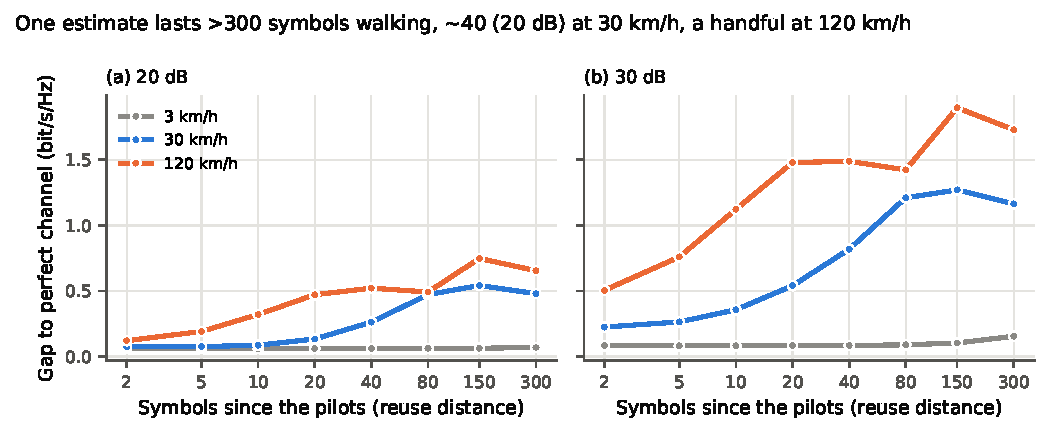
\includegraphics[width=0.8\columnwidth]{fig11_mobility.pdf}
\caption{Gap versus symbols since the pilots at 3, 30 and 120\,km/h (estimate reused).}
\label{fig:mob}\end{figure}
\begin{figure}[!htbp]\centering
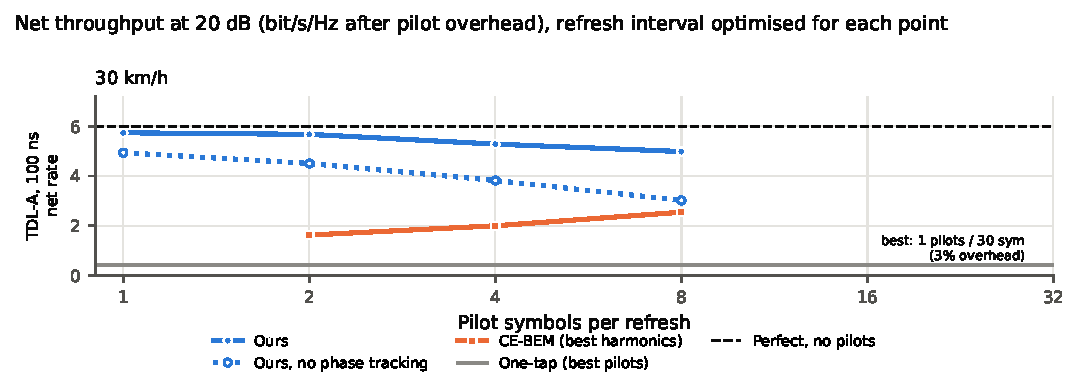
\includegraphics[width=0.85\textwidth]{fig19_pilot_overhead.pdf}
\caption{Net throughput at 20\,dB after pilot overhead versus pilot symbols per refresh.}
\label{fig:overhead}\end{figure}

\subsection{Measured cost}\label{sec:res-cost}
\emph{Updates for a moving user} ($M=256$, 30\,km/h, refresh every 20 symbols, 8 channels;
Table~\ref{tab:updates}). Warm start with two iterations needs 12$\times$ fewer operations than estimation
from scratch for 0.03\,bit/s/Hz more gap. Freezing $\bm V$ is about 100$\times$ cheaper and as good at 20\,dB,
but costs 0.23\,bit/s/Hz more at 30\,dB, because the rank-8 factorization does not split the static and
moving hops exactly; Algorithm~\ref{alg:learn} with $r=Q$ addresses this split. At the full band, a warm
update takes 1.4\,s against 12.5\,s from scratch in MATLAB (8.6$\times$), with the same SER (0.399 vs 0.398;
both estimates are 20 symbols old at 30\,km/h, which sets the absolute SER, see the caveat on tracking above).

\begin{table}[!htbp]\centering
\caption{Update variants for a moving user ($M=256$): gap at 20/30\,dB, operations, MATLAB time.}\label{tab:updates}
\begin{tabular}{lcccc}\toprule
Update & gap & operations & saving & time \\\midrule
From scratch, 20 it., $r=8$ & 0.07 / 0.17 & $1.2\cdot10^9$ & 1$\times$ & 307\,ms \\
From scratch, $r=6$ & 0.07 / 0.16 & $7.2\cdot10^8$ & 1.7$\times$ & 215\,ms \\
Warm start, 2 it. (Alg.~\ref{alg:warm}) & 0.10 / 0.20 & $1.0\cdot10^8$ & 12$\times$ & 31\,ms \\
$\bm V$ frozen, 1 it. & 0.10 / 0.40 & $1.1\cdot10^7$ & 105$\times$ & 8\,ms \\
$\bm V$ frozen, 1 pilot symbol & 0.13 / 0.49 & $6.0\cdot10^6$ & 197$\times$ & 5\,ms \\\bottomrule
\end{tabular}
\end{table}

\emph{Equalizer.} The pre-registered wall-clock comparison \emph{failed} with the element-by-element
FFT operator: at $M=3276$ CG with 25 iterations took 18.7\,s for 12 symbols against 5.6\,s for the dense
solve, with the same SER (0.065), because many small FFT calls are slow in MATLAB. With the batched
operator of Algorithm~\ref{alg:cg} and the stopping rule (a new pre-registered criterion), CG took
1.12\,s (5 iterations) against 2.95\,s dense at $M=3276$, 2.6$\times$ faster with the same SER, and
1.85\,s at $M=6552$, where the dense solve does not fit in memory (687\,MB per matrix). At $M=2048$ the
two are equal in time and the stopping rule left CG's SER 1.18$\times$ that of the dense solve, which
suggests a tighter tolerance there. The dense solve's time varied by 2$\times$ between runs with machine
load; comparisons are within a run (Fig.~\ref{fig:cost}).

\begin{figure}[!htbp]\centering
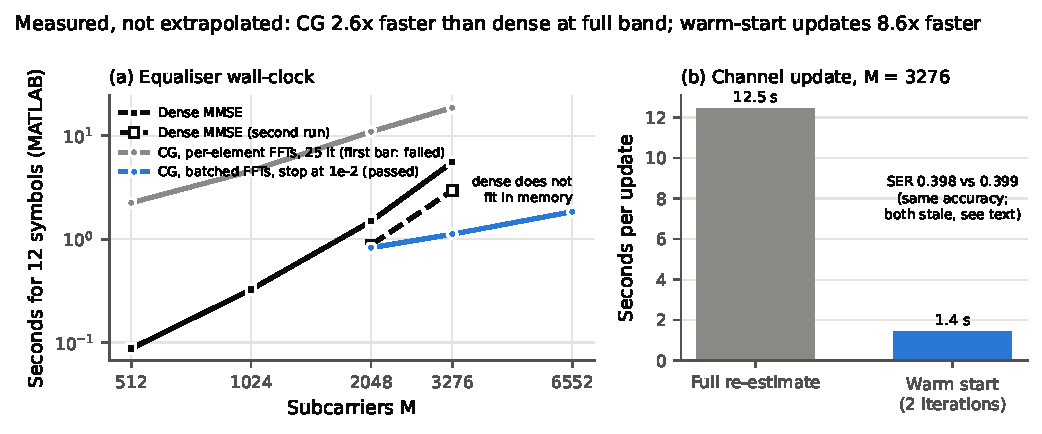
\includegraphics[width=\columnwidth]{fig22_compute_measured.pdf}
\caption{Measured equalizer time versus $M$ and full-band update time.}
\label{fig:cost}\end{figure}
